\documentclass[sigconf]{acmart}
\usepackage[spanish]{babel}

\AtBeginDocument{%
  \providecommand\BibTeX{{%
    \normalfont B\kern-0.5em{\scshape i\kern-0.25em b}\kern-0.8em\TeX}}}

\copyrightyear{2021}
\acmYear{2021}
\acmDOI{}

\acmConference{Motor de recomendación}{May 08, 2021}{Guatemala, Guatemala}
\acmBooktitle{Motor de recomendación, May 08, 2021, Guatemala, Guatemala}
\acmISBN{*}

\begin{document}

\title{Motor de Recomendación}

\author{Luis Chutá}
\affiliation{%
  \institution{Universidad Rafael Landívar}
  \state{Guatemala}
  \country{Guatemala}
  \postcode{01016}
}

\author{Walter Osoy}
\affiliation{%
  \institution{Universidad Rafael Landívar}
  \state{Guatemala}
  \country{Guatemala}
  \postcode{01016}
}

\author{Andres Gálvez}
\affiliation{%
  \institution{Universidad Rafael Landívar}
  \state{Guatemala}
  \country{Guatemala}
  \postcode{01016}
}

\author{Marcelo Rosales}
\affiliation{%
  \institution{Universidad Rafael Landívar}
  \state{Guatemala}
  \country{Guatemala}
  \postcode{01016}
}

\renewcommand{\shortauthors}{Chutá, L., et al.}

\begin{abstract}
The purpose of this article is to propose a probabilistic method of automatic classification of text according to its language, applying machine learning with supervised learning as a tool. The occurrence of each word in a certain language is captured and taken into account to establish its probability of coincidence. The training is given with a file loaded with a high volume of phrases with their respective labels, which allows covering a large number of words and avoiding repetition bias.
\end{abstract}

\begin{CCSXML}
<ccs2012>
 <concept>
  <concept_id>10010520.10010553.10010562</concept_id>
  <concept_desc>Computer systems organization~Embedded systems</concept_desc>
  <concept_significance>500</concept_significance>
 </concept>
 <concept>
  <concept_id>10010520.10010575.10010755</concept_id>
  <concept_desc>Computer systems organization~Redundancy</concept_desc>
  <concept_significance>300</concept_significance>
 </concept>
 <concept>
  <concept_id>10010520.10010553.10010554</concept_id>
  <concept_desc>Computer systems organization~Robotics</concept_desc>
  <concept_significance>100</concept_significance>
 </concept>
 <concept>
  <concept_id>10003033.10003083.10003095</concept_id>
  <concept_desc>Networks~Network reliability</concept_desc>
  <concept_significance>100</concept_significance>
 </concept>
</ccs2012>
\end{CCSXML}

\keywords{Naive Bayes, inteligencia artificial, machine learning, agente inteligente, clasificador de textos, Java}

\begin{teaserfigure}
 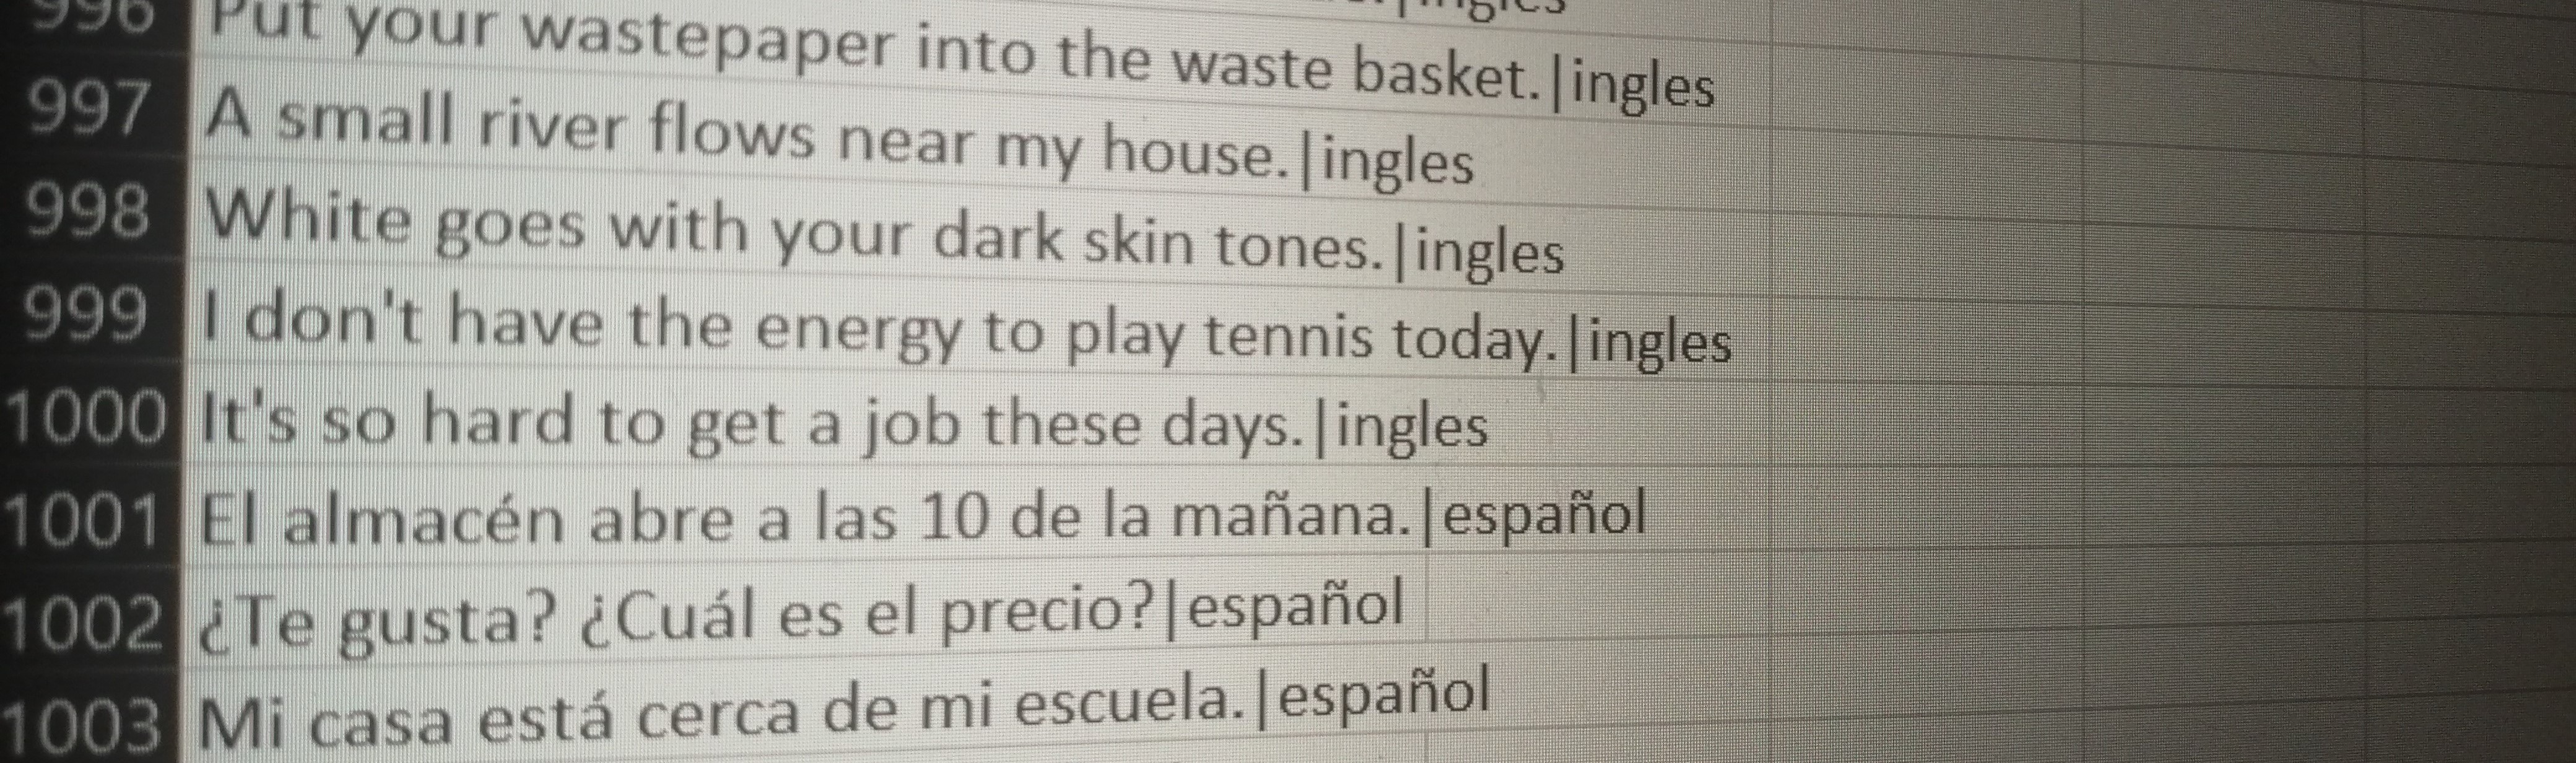
\includegraphics[width=\textwidth]{mainTeaser}
 \caption{Archivo de entrenamiento para la clasificación de texto.}
 \Description{Archivo con un gran volumen de datos que sirve de entrenamiento para el sistema.}
 \label{fig:teaser}
\end{teaserfigure}

\maketitle

\section{INTRODUCCIÓN}
La inteligencia artificial (IA) está cambiando la forma de trabajar y vivir. Se estima que la IA creará un valor de trece billones de dólares estadounidenses por año antes de 2030 y, aunque ya está creando una gran cantidad de valor dentro de la industria del software, una gran parte del valor que se estima estará fuera de esta, en sectores como ventas, viajes, transporte, manufactura y más.

El desarrollo de la IA ha sido impulsado, en gran parte, por una herramienta llamada {\itshape machine learning}. El tipo de {\itshape machine learning} más usado es un tipo de IA que aprende de A a B, es decir, asignación de datos de entrada a salida, también conocido como aprendizaje supervisado. Esta idea ha estado presente durante décadas, pero ha despegado en los últimos años debido al crecimiento exponencial de datos accesibles. En muchos sectores, la cantidad de datos a los que se tiene acceso ha crecido gracias al auge del internet y al desarrollo en la capacidad de procesamiento.

Una de las diversas aplicaciones de {\itshape machine learning} es la clasificación de texto, lo cual consiste en usar técnicas probabilísticas sobre un conjunto de elementos para asignarlos a grupos o categorías.  La clasificación automática de textos ha estado ligada históricamente al desarrollo  de máquinas de aprendizaje basadas en el desarrollo de algoritmos que «aprenden» o reconocen patrones recurrentes en cada clase a partir de un gran volumen textos de entrada, previamente clasificados por humanos.

En las siguientes secciones se introduce brevemente la teoría necesaria para abordar el manejo de los datos y la implementación de un agente inteligente capaz de clasificar textos según su idioma mediante estrategias probabilísticas, así como los resultados de su desempeño en dicha tarea. Finalmente, se presentan las conclusiones obtenidas de esta implementación.


\section{MARCO TEÓRICO}

\subsection{{\itshape Machine Learning}}
El aprendizaje automático, conocido generalmente como {\itshape machine learning}, hace referencia a la capacidad de un software de «aprender» mediante la adaptación de algoritmos respecto a una entrada de datos en su sistema ~\cite{apd}.

Concretamente, es una disciplina de las ciencias de la computación muy relacionada con la IA. Permite automatizar operaciones reduciendo la intervención humana para su funcionamiento, lo cual facilita el manejo efectivo de información masiva.

En la computación convencional, se define un algoritmo definido para que un sistema realice determinadas acciones. En {\itshape machine learning}, los algoritmos realizan muchas de las acciones por su cuenta, obteniendo sus propios cálculos según los datos que el sistema recopila, por esto es que, cuantos más datos se obtengan, mejor será el entrenamiento y más precisas serán las acciones resultantes.

\subsubsection{Tipos de {\itshape Machine Learning}} Existen tres tipos principales de {\itshape machine learning}:

\begin{itemize}
    \item Aprendizaje supervisado \newline
    Se basa en información de entrenamiento. Se entrena al sistema mediante un volumen de datos definidos y clasificados previamente. Así, el sistema podrá inferir mediante los patrones registrados durante el entrenamiento.
    \item Aprendizaje no supervisado (clustering) \newline
    En este modelo, no se usan etiquetas, pues la finalidad del sistema es la abstracción de patrones de manera directa. Este es un modo de entrenamiento más apegado al procesamiento humano de información.
    \item Aprendizaje por refuerzo \newline
    Toma la experiencia como base. Es un sistema de «premios y castigos» que actúa bajo el esquema de prueba y error.
\end{itemize}

\subsection{Clasificación de Texto}
Hasta ahora ha habido numerosas propuestas para la clasificación. Una de las más extendidas, sobre todo por su simpleza, es «Bolsa de palabras» (bag of words, $BoW$). La representación $BoW$ forma un arreglo con la frecuencia de los términos, o variables predictoras presentes en el texto. Sin embargo, carece de información sobre relaciones entre estos términos, así como de relaciones semánticas que existen entre estos. Frente a esta simplificación, otras representaciones que consideran el peso estadístico en las frecuencias de los términos, o que mediante ontología rescatan las relaciones semánticas entre estos, también han sido propuestas ~\cite{scielo}. 

Con un enfoque distinto, también se ha propuesto una representación que transforma el texto en un grafo dirigido, donde los nodos corresponden a palabras y los enlaces a sus relaciones.

Es necesario remarcar que si bien cada una de estas representaciones supone un aporte, también presentan sus propias limitaciones, ya sean de implementación, de complejidad computacional o de requerimientos de memoria.

Bajo el marco formal del aprendizaje supervisado, se define como $D$ el espacio de entrada que representa los textos y $C$ el espacio de salida de un proceso de clasificación realizado por un humano, donde cada par $(d_{i},c_{i})$ corresponde a una frase y la categoría en la que este fue clasificado, respectivamente. Así mismo, se define $Z$ como el conjunto de estos pares de textos y sus clasificaciones, $z_{i}=(d_{i}, c_{i})$.

\subsection{Algoritmos clasificadores}
Así como sucede con las representaciones, muchos clasificadores de textos también han sido propuestos, como las Máquinas de Soporte Vectorial ($SVM$). Estas corresponden a máquinas de aprendizaje que toman distintas características de los elementos que se quieren clasificar y los llevan a un espacio vectorial multidimensional. Es en este espacio, donde el algoritmo identifica, de forma óptima, un hiperplano que separa a los vectores de una clase del resto. Es en ese concepto de separación óptima donde reside la característica fundamental de estos algoritmos. 

Otros clasificadores de texto destacados son el clasificador de vecinos próximos, los árboles de decisión y las redes neuronales. Todos estos, al igual que {\itshape Naive Bayes}, el cual se destaca a continuación por ser el clasificador a implementar, y las $SVM$, usan por lo general representaciones vectoriales de texto tales como $BoW$.


\subsection{{\itshape Naive Bayes}}
En un sentido amplio, los modelos de {\itshape Naive Bayes} son una clase especial de algoritmos de clasificación de {\itshape machine learning}. Se basan en una técnica de clasificación estadística llamada «Teorema de Bayes».

En este punto se asume que las variables predictoras son independientes entre sí, es decir que la presencia de una cierta característica en un conjunto de datos no está en absoluto relacionada con la presencia de cualquier otra característica ~\cite{vRoman}.

El más simple de los clasificadores de texto propuestos es {\itshape Naive Bayes}, correspondiente a un modelo estructural y a un conjunto de probabilidades condicionales. La estructura del modelo es la de un grafo dirigido en el que cada nodo representa un atributo y cada enlace representa la dependencia entre atributos expresada por una probabilidad condicional por cada nodo.


\subsubsection{Teorema de Bayes} Llamado así por el inglés Thomas Bayes. Describe las alternativas para calcular la probabilidad de que eventos sucedan, usando los principios de la probabilidad condicional y juicios a partir de datos incompletos. 

El teorema de Bayes es aplicable a todas las cuestiones relacionadas con el aprendizaje a través de la experiencia. Su ecuación característica se define como

\begin{equation}
    P(A|B)=\frac{P(B|A) * P(A)}{P(B)}
\end{equation}

donde $P(A|B)$ es la probabilidad de que ocurra un suceso $A$ dado una evidencia $B$, $P(B|A)$ es la probabilidad de que ocurra un suceso $B$ dada una evidencia $A$, $P(A)$ es la probabilidad independiente de que ocurra un suceso $A$ y $P(B)$ es la probabilidad independiente de que ocurra un suceso $B$.

\subsubsection{{\itshape Naive Bayes supervisado}}
\begin{itemize}
    \item Se debe convertir el conjunto de datos en una tabla de frecuencias.
    \item Se debe crear una tabla de probabilidad calculando las correspondientes a que ocurran los diversos eventos.
    \item Se calcula la probabilidad posterior de cada clase.
    \item La clase con la probabilidad posterior más alta es el resultado de la predicción.
\end{itemize}

\subsubsection{Puntos fuertes de {\itshape Naive Bayes}} 
\begin{itemize}
    \item Es una manera sencilla de predecir clases para problemas de clasificación binarios y multiclase.
    \item En los casos donde es apropiada una presución de independencia, el algoritmo se desempeña mejor que otros modelos de clasificación, incluso con menor volumen de datos de entrenamiento.
    \item El desacoplamiento de las distribuciones de características condicionales de clase significan que cada distribución puede ser estimada independientemente como si tuviera una sola dimensión, logrando mejorar así el rendimiento.
\end{itemize}

\subsubsection{Puntos débiles de {\itshape Naive Bayes}}
\begin{itemize}
    \item Es conocido por ser un estimador pobre, por lo que las probabilidades obtenidas no pueden tomarse como totalmente certeras.
    \item Es muy probable que presunción de independencia no refleje cómo son los datos en el mundo real.
    \item Cuando el conjunto de datos de prueba tiene una característica que no ha sido observada en el conjunto de entrenamiento, el modelo le asignará una probabilidad de cero y realizar predicciones será inútil. Uno de los principales métodos para evitarlo es la técnica de suavizado, siendo la estimación de Laplace una de las más populares.
\end{itemize}

\begin{figure}[h]
  \centering
  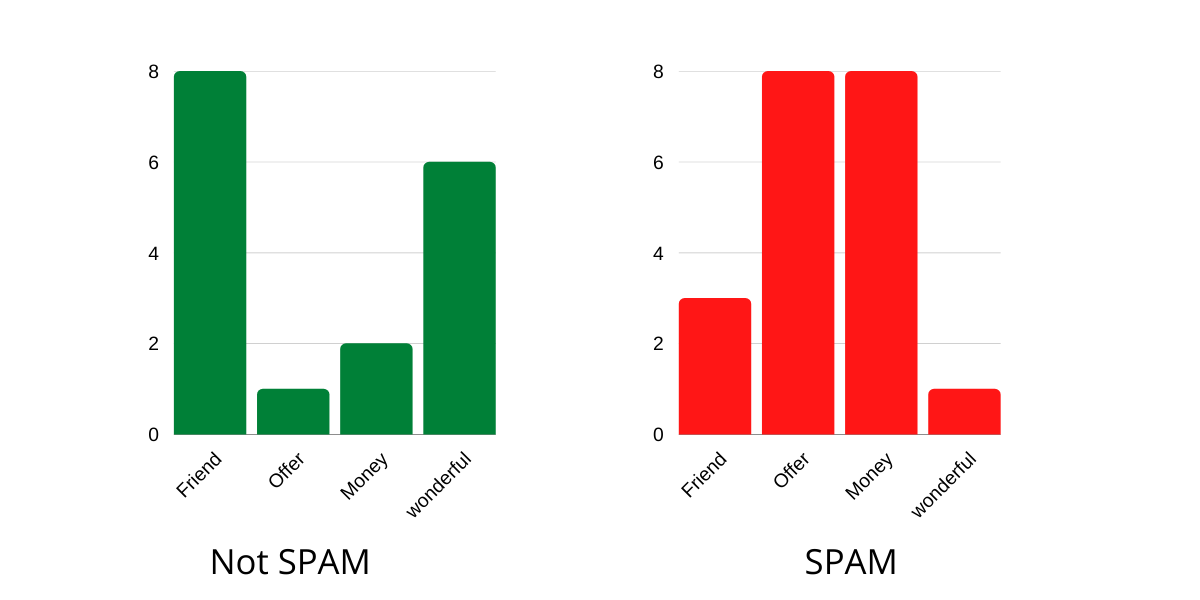
\includegraphics[width=\linewidth]{spamNaive}
  \caption{Clasificación de correos electrónicos según la probabilidad de aparición de determinadas palabras. (\url{https://www.askpython.com/python/examples/naive-bayes-classifier}).}
  \Description{Dos gráficos que muestran el conteo de determinadas palabras en correos clasificados como spam y no spam.}
\end{figure}

\section{MARCO METODOLÓGICO}
\subsection{Lenguaje de programación y entorno de desarrollo integrado (IDE)}
El sistema propuesto está escrito en lenguaje de programación Java, dada su capacidad multiplataforma, robustez, la orientación a objetos y la corta curva de aprendizaje que supone. Está codificado gracias a IntelliJ IDEA.

\begin{figure}[h]
  \centering
  
\includegraphics[width=50]{intellij}
  \caption{Ícono del IDE.}
  \Description{Un cuadro que muestra el ícono del estudio empleado.}
\end{figure}

\subsection{Modelo}
Como modelo se toma {\itshape naive Bayes}, aprovechando su simpleza. Cabe mencionar que este modelo se construye desde cero, sin usar ninguna librería o código prefabricado, con el objetivo de explorar distintas variaciones convenientes al problema a resolver y profundizar en la lógica.

\subsection{Entrenamiento}
Para entrenar al sistema, se propone la carga de un archivo CSV con un alto volumen de frases clasificadas en distintos idiomas, lo cual permitirá la creación del modelo probabilístico.

\subsection{Utilidades adicionales}
Por su parte, se plantea también el uso de una base de datos que sirve como almacenador de palabras por idioma, facilitando el procesamiento en memoria del equipo.

\section{RESULTADOS OBTENIDOS}
\subsection{Interfaz de usuario}
Se desarrolló una interfaz de usuario en consola, incluyendo un menú de opción numérica y validación de errores de entrada.

\begin{figure}[h]
  \centering
  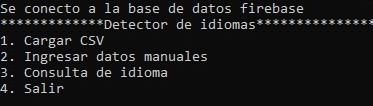
\includegraphics[width=\linewidth]{menu}
  \caption{Interfaz en consola con el menú de usuario.}
  \Description{Una consola con un menú de acciones para el usuario.}
\end{figure}

\subsection{Base de datos}
El sistema se conecta con una base de datos de Firebase, con la finalidad de almacenar las palabras leídas durante el entrenamiento con su respectivo conteo.

\begin{figure}[h]
  \centering
  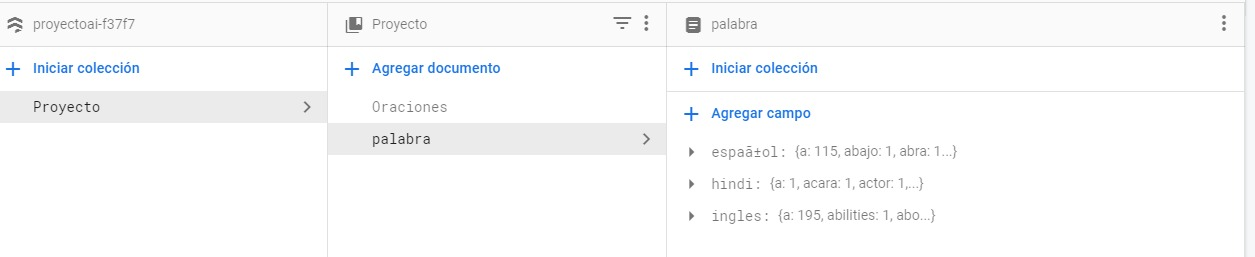
\includegraphics[width=\linewidth]{bd}
  \caption{Vista del almacenamiento de datos en Firebase.}
  \Description{Demostración del almacenamiento de los datos fuera del ambiente del sistema.}
\end{figure}

\subsection{Entrenamiento}
El entrenamiento se dio mediante la carga al sistema de un archivo CSV, tal cual se indicó en la sección anterior.

\begin{figure}[h]
  \centering
  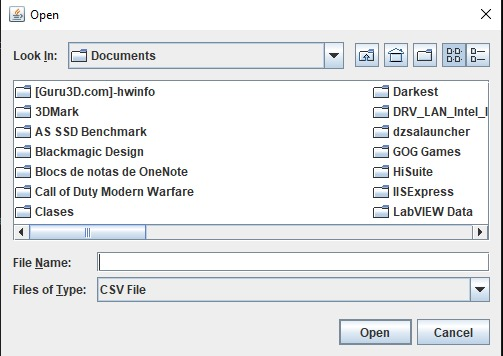
\includegraphics[width=\linewidth]{csv}
  \caption{Vista de la carga del archivo de entrenamiento.}
  \Description{Explorador de archivos.}
\end{figure}

\subsection{Inferencia}
Aplicando efectivamente el modelo creado y entrenando al sistema, es posible predecir y mostrar la probabilidad de certeza (dada en decimal) de la pertenencia de una frase a un determinado idioma.

Para esto, se realiza una consulta a la base de datos donde se cargó toda la información de entrenamiento, para armar probabilidades y llegar al resultado.

\begin{figure}[h]
  \centering
  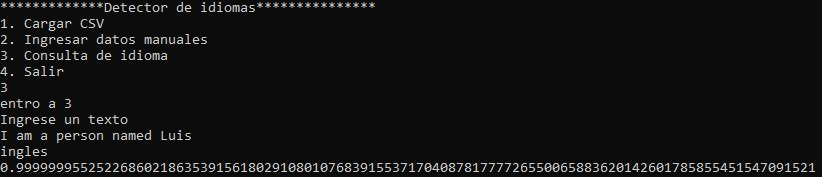
\includegraphics[width=\linewidth]{inferencia}
  \caption{Vista de la carga del archivo de entrenamiento.}
  \Description{Explorador de archivos.}
\end{figure}

\bibliographystyle{ACM-Reference-Format}
\bibliography{main-ref}

\section{CONCLUSIONES}
\begin{itemize}
    \item La inteligencia artificial tiene un auge en los últimos años gracias al crecimiento de datos y a la facilidad de acceso a ellos, impulsado por el internet.
    \item A pesar de que {\itshape naive Bayes} se caracteriza como un modelo simple, es eficaz en pequeñas predicciones en agentes inteligentes que no requieren realizar tareas complejas.
    \item En los sistemas de {\itshape machine learning}, el volumen de datos de entrenamiento juega un papel importante en su desempeño. Mientras más completos sean estos datos, más efectivo será el resultado.
\end{itemize}

\section{AGRADECIMIENTOS}
A la Universidad Rafael Landívar, por una educación basada en la excelencia académica con valores y al Ing. Msc. Víctor Orozco, por su labor docente en el curso Inteligencia Artificial.

\end{document}
\endinput